
\documentclass{article}

% If you're new to LaTeX, here's some short tutorials:
% https://www.overleaf.com/learn/latex/Learn_LaTeX_in_30_minutes
% https://en.wikibooks.org/wiki/LaTeX/Basics

% Formatting
\usepackage[utf8]{inputenc}
\usepackage[margin=1in]{geometry}
\usepackage[titletoc,title]{appendix}

% Math
% https://www.overleaf.com/learn/latex/Mathematical_expressions
% https://en.wikibooks.org/wiki/LaTeX/Mathematics
\usepackage{amsmath,amsfonts,amssymb,mathtools}

% Images
% https://www.overleaf.com/learn/latex/Inserting_Images
% https://en.wikibooks.org/wiki/LaTeX/Floats,_Figures_and_Captions
\usepackage{graphicx,float}

% Tables
% https://www.overleaf.com/learn/latex/Tables
% https://en.wikibooks.org/wiki/LaTeX/Tables

% Algorithms
% https://www.overleaf.com/learn/latex/algorithms
% https://en.wikibooks.org/wiki/LaTeX/Algorithms
\usepackage[ruled,vlined]{algorithm2e}
\usepackage{algorithmic}

% Code syntax highlighting
% https://www.overleaf.com/learn/latex/Code_Highlighting_with_minted
\usepackage{minted}
\usemintedstyle{borland}

% References
% https://www.overleaf.com/learn/latex/Bibliography_management_in_LaTeX
% https://en.wikibooks.org/wiki/LaTeX/Bibliography_Management
\usepackage{biblatex}
\addbibresource{references.bib}
\usepackage[euler]{textgreek}
\usepackage{url}
\usepackage{hyperref}
\usepackage{float}
\usepackage{siunitx}
\renewcommand \thesubsubsection {\Alph{subsubsection}}
\renewcommand{\thesubsubsection}{\alph{subsubsection})}
\makeatletter
\renewcommand{\p@subsubsection}{\thesubsection.\protect\eatbracket}


% Title content
\title{EE 462 Homework 1}
\author{Burak Kemal Kara}
\date{March 21, 2020}

\begin{document}
\begin{titlepage}
    \begin{center}
        \vspace*{1cm}
            
        \Huge
        \textbf{DC/DC Voltage Regulator}
            
        \vspace{0.5cm}
        \LARGE
        Complete Simulation Report
            
        \vspace{1.5cm}
            
        \textbf{Cemil Ürgüp}\\
        \textbf{Burak Kemal Kara}
            
        \vfill
            
        A report presented for the sake of\\
        Humanity and Science
            
        \vspace{0.8cm}
            
        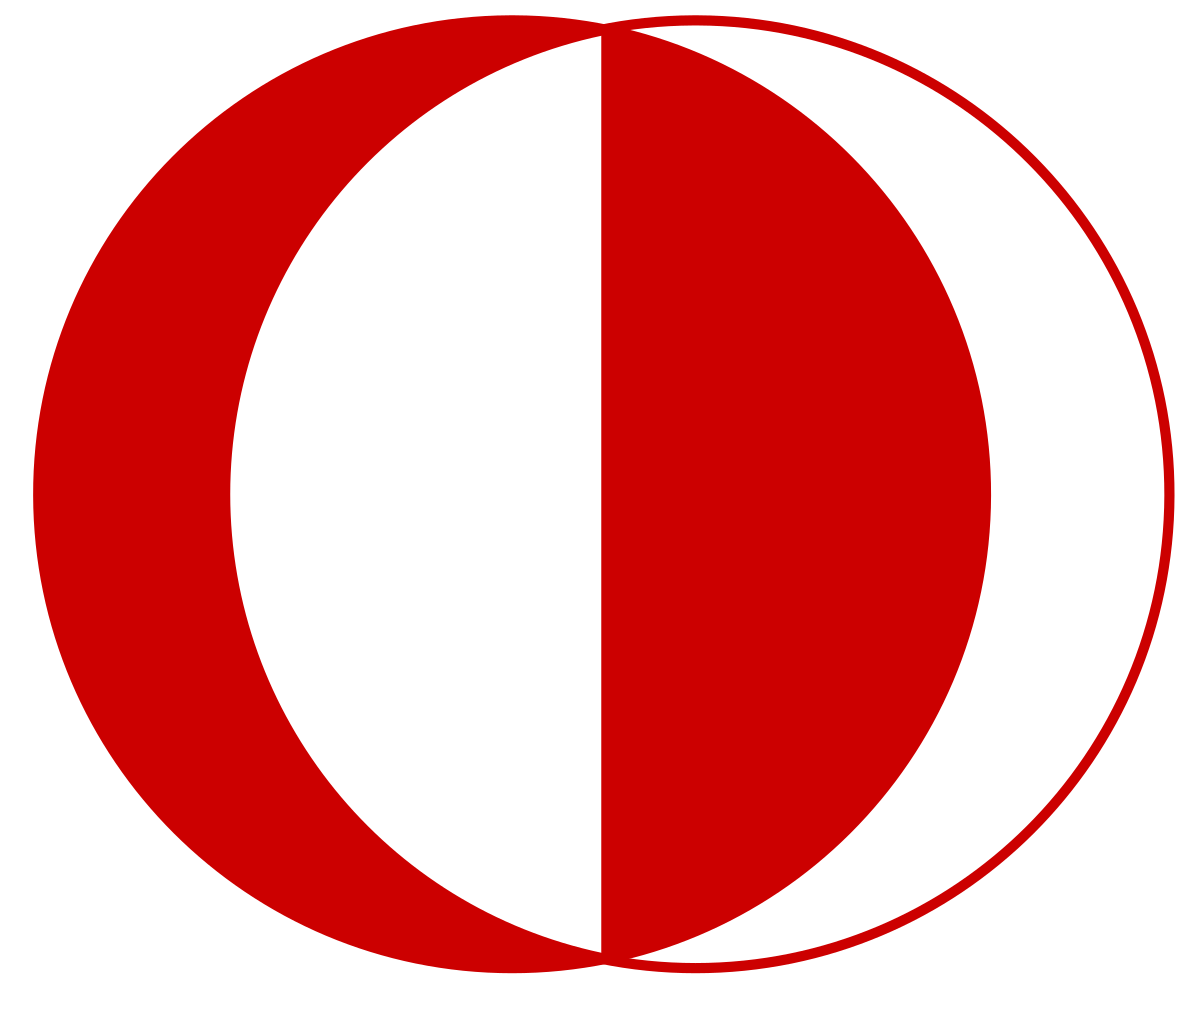
\includegraphics[width=0.4\textwidth]{logo.png}
            
        \Large
        Electrical \& Electronics Engineering\\
        MIDDLE EAST TECHNICAL UNIVERSITY\\
        TURKEY\\
        23.03.2020
            
    \end{center}
\end{titlepage}
%Table of contents
\tableofcontents
\newpage
%Introduction
\section{Introduction}
Switch mode power supplies are commonly used to DC/DC converter applications. 
Beside of voltage control, it provides galvanic isolations. 
In this project we used Forward Converter topology which is good choice when output need high current and power range is below 200W. 
In addition, UC3844 IC is examined and simulated in order to obtain constant output voltage with current control.
This document aims to discuss component selections,cost and power estimation according to teoric and computational simulation results.
\section{Forward Converter topology}
Forward converter topology is derived from buck converter, at each cycle input transfer power to load side. To avoid saturation at core we choose to use reset windigs.Details are shown Figure ~\ref{fig:topology}.
\begin{figure}[H]
    \centering
    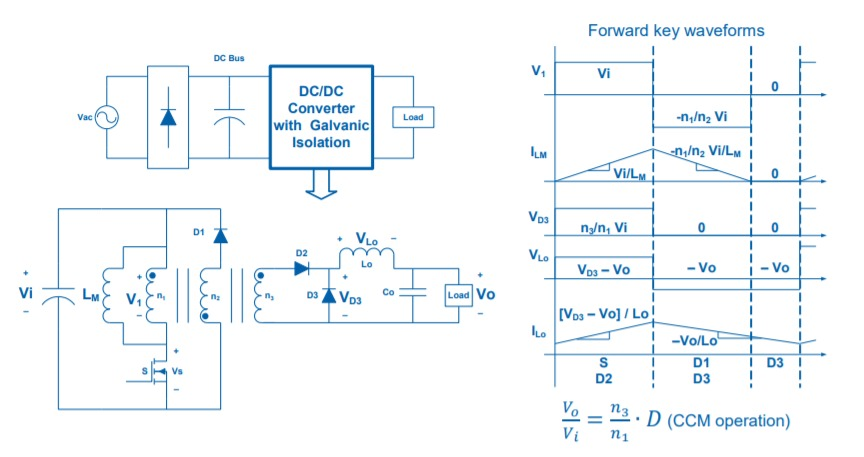
\includegraphics[width=0.8\linewidth]{topology.jpeg}
    \caption {Diagram,schematic and basic waveforms for Forward converter with reset winding cited \cite{topology}}
    \label{fig:topology}
\end{figure}
In this project, we had different design options as can be seen from Figure ~\ref{fig:projects}.
\begin{figure}[H]
    \centering
    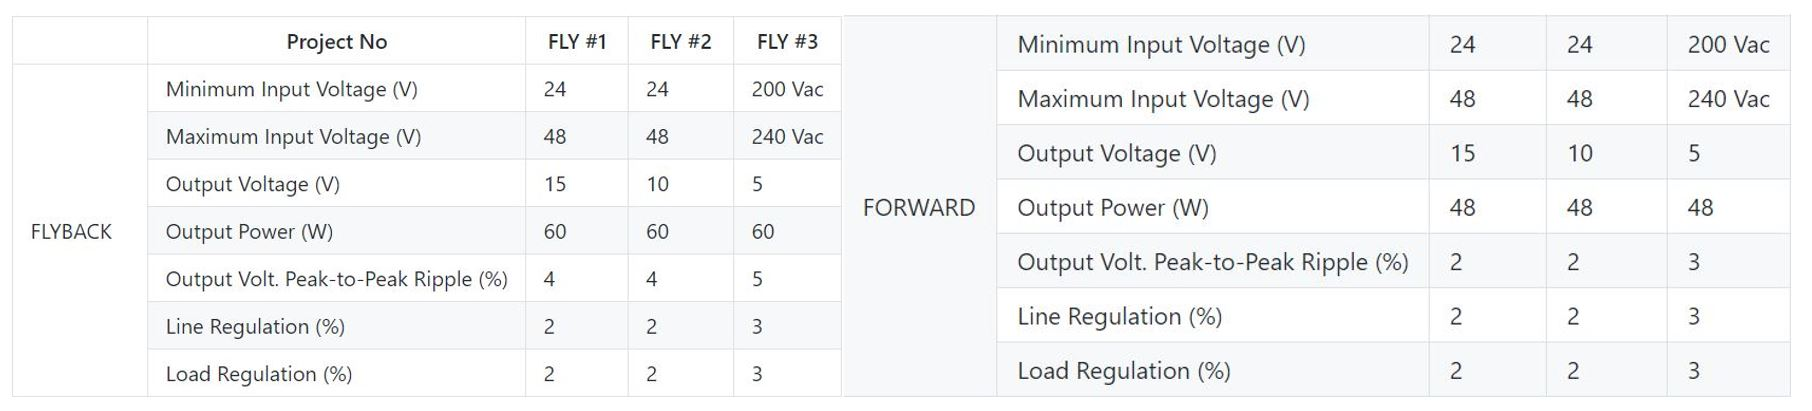
\includegraphics[width=1\linewidth]{projects.jpeg}
    \caption {Different Design alternatives of the project}
    \label{fig:projects}
\end{figure}

From these alternatives, Forward \#1 option is selected. Although, Forward Converter has more components and it is more complex than Flyback Converter, it has some important advantages over Flyback converter such as:
\begin{itemize}
    \item It has better transformer utilization. It transfers its energy instantly across the transformer and it does not need energy storage element in transformer. For that reason, transformer can be more ideal with higher magnetizing inductance and no air gap
    \item Output inductor and freewheeling diode ensure continuous output current and it causes less ripple at the output. Furthermore, since main energy storage element is inductor, output capacitor can be smaller than flyback.
    \item It has less voltage and current stresses on switching components because of larger magnetizing inductance.
\end{itemize}
Disadvantages of Forward Converter compared to Flyback:
\begin{itemize}
    \item It is more expensive than flyback because of extra freewheeling diode and output inductor.
    \item It has minimum load requirements because gain changes a lot in DCM operations
\end{itemize}

\section{Design Equations}
The following specifications are design equtions for Forward Converter Design.
\begin{table}[H]
    \centering
\begin{tabular}{|l|l|}
    \hline
    Minimum Input Voltage (V)             & 24      \\ \hline
    Maximum Input Voltage (V)             & 48      \\ \hline
    Output Voltage (V)                    & 15      \\ \hline
    Output Power (W)                      & 48      \\ \hline
    Output Volt. Peak-to-Peak Ripple (\%) & 2       \\ \hline
    Switching Frequency (fs)              & 100 kHz \\ \hline
\end{tabular}
\caption {Design specifications}
\end{table}
%Transformer
\subsection{Transformer Considerations}
First of all we should calculate turn ratio of transformer. For the sake of simplicity reset winding and primary winding ratio is same.
\begin{equation}
    n_{1}=n_{3}
\end{equation}
This equation limit max duty ratio to 50\%, since core cant demagnetize faster than magnetizing time.
Primary and secondary winding ratio can found when critical points are considered. When Input decreased minumum, Duty cycle reached max. ratio.At this point this converter should supply desired $V_o$.
\begin{equation}
    V_o<v_i\frac{n_3}{n_1}D \quad \implies \quad \frac{n_3}{n_1}>\frac{V_o}{V_i\cdot D}=1.33 \implies 2
\end{equation}
When $V_o=15 V$ as specifications, extra voltage drop on $D_2$ around 1V. \\$V_{o,max}=16 V$.\\Minimum voltage is 24 V. \\Maximum D is 50\%.\\
At this point we choose R type material ferrite core (Code:0R45959EC). We selected since,R type core loss is less than P type core. According to this core turning factor can found from Lenz Rule,
\begin{equation}
    V=n_1\frac{d\phi}{dt} \implies V_{i,max}=\frac{n_1\cdot B_{sat}\cdot A_e}{D{max}\cdot T_s}
\end{equation}
\[\therefore n_1> 2.18\]
$V_{i,max}$=48 V\\
$D_{max}$=0.5\\
$B_{sat}$=0.3\\
$A_e= 368 mm^2$ taken from datasheet \cite{core}.\\
This is minimum turning ratio to avoid core saturation.
To calculate max turn number we should calculate wire type to know wire size.
At the worst scenario we have $V_{in,min}=24 V$. For primary winding,
\begin{equation}
    I_{primary}=\frac{P_o}{V_{in,min}}=2A
\end{equation}
For secondary winding,
\begin{equation}
    I_{secondary}=\frac{I_{primary}}{n}=1A
\end{equation}
Since this currents ratings are for ideal case, it is safer to choose higher rating wires.From AWG chart,for primary and reset windings can use AWG \#16, Secondary AWG \#18. Selection criteria is max current. Their properties are shown at table 2.
\begin{table}[H]
    \centering
\begin{tabular}{|l|l|l|}
    \hline
    \multicolumn{1}{|c|}{AWG} & \multicolumn{1}{c|}{\begin{tabular}[c]{@{}c@{}}Area\\ mm\textasciicircum{}2\end{tabular}} & \multicolumn{1}{c|}{\begin{tabular}[c]{@{}c@{}}Max. Current \\ Amperes\end{tabular}} \\ \hline
    AWG\#16                   & 1.31                                                                                      & 3.7                                                                                  \\ \hline
    AWG\#18                   & 0.823                                                                                     & 2.3                                                                                  \\ \hline
    \end{tabular}
    \caption{Wire properties}
\end{table}
Core window area is calculated from datasheet.Also geometry parameters are taken from datasheet \cite{core}.
\begin{equation}
    A_{w}=(E-F)\cdot D=510 mm^2
\end{equation}
Since area of wires are known max turn can be calculate by,
\begin{equation}
    N_{max}=\frac{k_{fill}\cdot A_w}{A_{pri}+n\cdot A_{sec}+A_{reset}}=71.73
\end{equation}
Note that fill factor is 0.3 for litz wire.Increasıng turn is good because flux density decreasing and core loss decreasing according to Steinmetz equation, but increased turn also increase resistance of wire and copper loss increased.
Core loss equation,
\begin{equation}
    P_{fe}=K_{fe}(B_{peak})^\beta A_cl_m
\end{equation}
$P_{fe}$ at 100kHz,100mT given $85mW/cm^3$\\
$P_{fe}$ at 100kHz,200mT given $550mW/cm^3$\\By using these values steinmetz parameters calculated as,\\
\[\therefore \beta =2.7 \quad ,K_{fe}=42\]
Core loss is simply $I^2R_{ac}$ but wires new resistance should be calcualted by skin effect.Since skin depth decrease wire area new resistance calculated by,
\begin{equation}
    R_{ac}=\frac{n\cdot MLT \cdot \rho}{Area }
\end{equation}
To find optimum turn number loss calculated at matlab script which provided at github repo.
\begin{figure}[H]
    \centering
    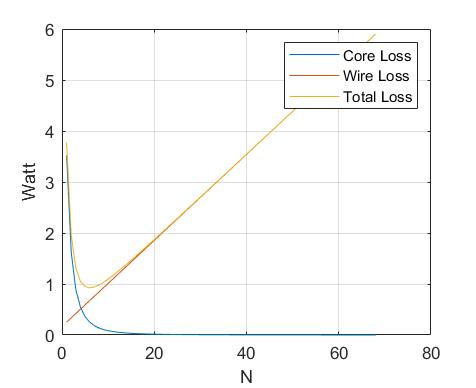
\includegraphics[width=0.5\linewidth]{number.jpg}
    \caption {According to number of turn Total loss calculated}
    \label{fig:sepic_cap_ideal}
\end{figure}
It is better to select turn ratio 8 which Total loss is 1 Watt.
At this number $R_{pri}=R_{reset}=0.05 k\Omega$, $R_{sec}=0.06 k\Omega$.\\
By using AL number windings inductance found and,
\begin{equation}
    X_m=k\cdot \sqrt{X_1\cdot (X_2+X_3)}=637 \mu H 
\end{equation}
Since reset and secondary windings direction same they summed. Also from Steinmetz eqn. $R_m$ can found.Where applied voltage is 48 V.
\begin{equation}
    P_{fe}=0.1375 Watt \implies R_m=\frac{V^2}{P_{fe}}=16.7k\Omega
\end{equation}
\subsection{MOSFET Considerations}
Since when switch is off, reset windig decharge core, beside of input voltage additional voltage seen on mosfet.
\begin{equation}
    V_s=V_i+\frac{n_1}{n_2}\cdot V_i=96 V
\end{equation}
For the worst case, selected $V_i=48V$. To be stay at the safe side lets make it 150V.
We aims to work in \%90 efficiency.Since $P_o=48 W$, $P_i=54 W$.At the minimum voltage max current created.
\begin{equation}
    I_i=\frac{P_i}{V_i}=2.22 A
\end{equation}
To be safe side minimum current of mosfet should be 5 A.
We selected to use IRF 740 N \cite{mosfet}, its voltage is 400V but since it has low resistance and it presents at available component list at the laboratory it is advantageous.
\\According to datasheet turn on and turn off time is 45ns.This much smaller than switching $t_off$ and $t_off$.
\begin{equation}
    P_{cond}=I_{i}^2\cdot R_{on}=2.7 W
\end{equation}
\begin{equation}
    P_{switching}=\frac{1}{2}\cdot V_{in}I_{in}(t_r+t_f)f_s=0.12W
\end{equation}
Conduction power loss is higher than expect, We can change this mosfet with better one at future. We will use this mosfet since we already have this component at the laboratory.
Lets use heatsink,Model No. :M-C092. Its Rca=3C/W. MOSFET Rth is 0.52.Assume enviroment temperature is 30C. Thus,
\begin{equation}
    T_j=C_{normal}+P_{total}\cdot (Rca_{heatsink}+ Rca_{mosfet})=49.2 Celcius.
\end{equation}
\subsection{Output Inductor Considerations}
Since \%2 voltage ripple, current change is $I_{ripple}=0.02\cdot \frac{P_o}{V_o}=0.064 A$Assume we apply 48 V input, and capacitor is big enough to constat output,
\begin{equation}
    V_L=L\frac{di}{dt} \implies nV_i-V_o=L\frac{I_{ripple}}{DT_s}=130\mu H
\end{equation}
\[\therefore L>130\mu H\]

We considered ripple voltage limit in our simulations and we chose 470 µH inductor according to our simulations. In addition, previous 10 A current rating selection must be valid for inductor. Therefore, we picked an inductor with 10 A maximum DC current and 470 µH inductance which is “CG3885-ALB” inductor from Coilcraft. It has also 8 mΩ maximum DC resistance and we used that value in our simulations.
Since inductors has nonideal series resistance values, there are power losses of these resistance values also. CG3885-ALB inductor has 8 mΩ resistance and it has 3.2 A current. Therefore, power losses on inductor can be calculated as follows:
\begin{equation}
    P_{inductor}=I^2\cdot R=3.2^2\cdot 8\cdot 10^-3=0.08W
\end{equation}

\subsection{Capacitor Considerations}
When $V_in=48 V$, D=0.156,
\begin{equation}
    \textDelta V=V_{ripple}=\frac{V_o}{50}=0.3V
\end{equation}
\begin{equation}
    \textDelta Q=C\textDelta V
\end{equation}
\begin{equation}
    I_oDT_s=CV_{ripple}
\end{equation}
\[\therefore C>16\mu F\]
Because of ripple voltage limit, we chose 150 µF capacitor. In addition, we select voltage rating of capacitor as 50 V because of safety limit and possibility of voltage oscillation in case of soft start does not working. Therefore, we picked “860080675012” capacitor from Würth Elektronik \cite{capacitor}.From datasheet impedance at 100kHz is $0.068\Omega$.
\begin{equation}
    impedance=ESR+\frac{1}{jwC} \implies ESR=0.05 \Omega
\end{equation}

\subsection{Diode Considerations}
As can be seen from Figures ~\ref{fig:soft}, there are 100 Volts when diodes are OFF and there are 3.2 A current when they are ON. Therefore, because of safety margin and high current possibility at the starting we chose 200 V and 10 A ratings for diodes. Hence, we picked “DPG10I200PM” \cite{diode} fast recovery diodes. For diodes another important parameter is reverse recovery time and this diode has 35 ns which is enough for 100 kHz frequency applications.
\begin{figure}[H]
    \centering
    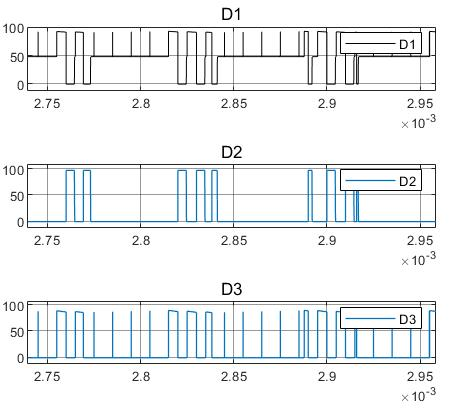
\includegraphics[width=0.5\linewidth]{diodes.jpg}
    \caption {Diodes}
    \label{fig:diodes}
\end{figure}
Output diodes has 0.98 V voltage drop and at steady state their current will be 3,2 A. When one diode is ON the other diode is OFF at the output. Therefore, we can calculate conduction losses by simply multiply voltage drop and forward current.
\begin{equation}
    P_{conduction}=V_fI_f=0.98V\cdot 32A=3.13 W
\end{equation}
For calculating switching losses of diodes, reverse recovery charge, blocking voltage and switching frequency is needed. From Figure ~\ref{fig:diode_loss}, we can estimate our reverse recovery charge as 0.1 µC. Blocking voltage is 100 V from simulations and switching frequency is 100 kHz.
\begin{figure}[H]
    \centering
    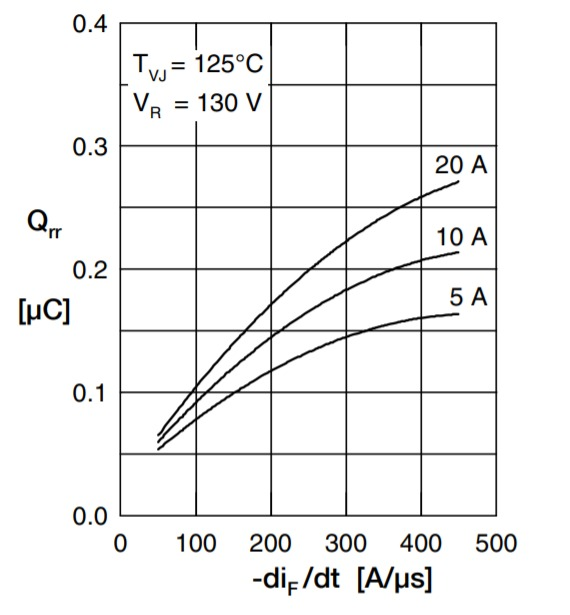
\includegraphics[width=0.5\linewidth]{diode_loss.jpeg}
    \caption {Reverse recovery charge values of DPG10I200PM}
    \label{fig:diode_loss}
\end{figure}
From these values, switching losses of two diodes can be calculated as follows:
\begin{equation}
    P_{switching}=Q_RV_Rf_s=2\cdot 0.1\cdot 10^-6\cdot 100V\cdot 100kHz=2W
\end{equation}
\section{Aimed Bonuses}
\subsection{Analog Controller IC}
We are planning to use UC3844 \cite{uc3844} High Performance Current Mode Controller. It also has soft start option if proper external circuitry is designed.
In Simulink, we established current mode control by using inner circuitry of this IC by oscillator and error amplifier and it worked as we want.This IC also allows us to ensure that our converter operates in line and load regulations limits because of feedback. In case of any change on the load or input, IC senses that change and regulates output voltage with very high accuracy.
\subsection{Efficiency Bonus}
As simulated at matlab efficiency is \%85.We try to select components to decrease loss and increase efficiency.
\subsection{Current Mode Control}
Current control Mode control decrease oscillations and output reach steady state faster.
\begin{figure}[H]
    \centering
    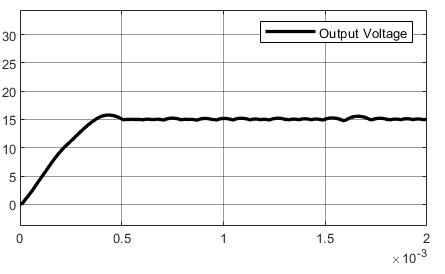
\includegraphics[width=0.5\linewidth]{voltage_control.jpg}
    \caption {Voltage Controlled mode Output Voltage}
    \label{fig:voltage_control}
\end{figure}
\begin{figure}[H]
    \centering
    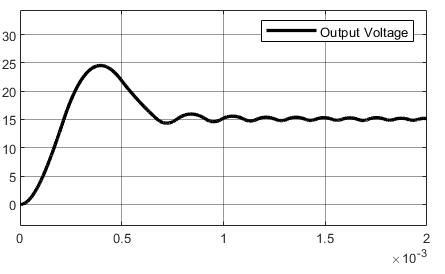
\includegraphics[width=0.5\linewidth]{current_control.jpg}
    \caption {Current Controlled mode Output Voltage}
    \label{fig:current_control}
\end{figure}
As seen Current control mode reach steady state faster than voltage control.
\subsection{PCB}
We are planning to implement our final circuitry on Printed Circuit Board (PCB). Because PCB has some advantages over stripboard. It is more professional than stripboard and it is less noisy. Also, after drawing proper PCB layout it is easy to implement.
\subsection{Soft Starting}
Soft starting is important issue for such applications because at the very beginning of implementation circuit has tendency to draw much more current than steady state. Reason of this problem is energy storage devices in the circuit. Until capacitors and inductor reaches steady state, they draw more current and that is why soft starting is needed. Since it is not desired, most of the controller ICs have soft starting feature and UC3884 also has this feature. For using soft starting mode of our IC, simple circuitry that can be seen in Figure ~\ref{fig:soft} is enough.
\begin{figure}[H]
    \centering
    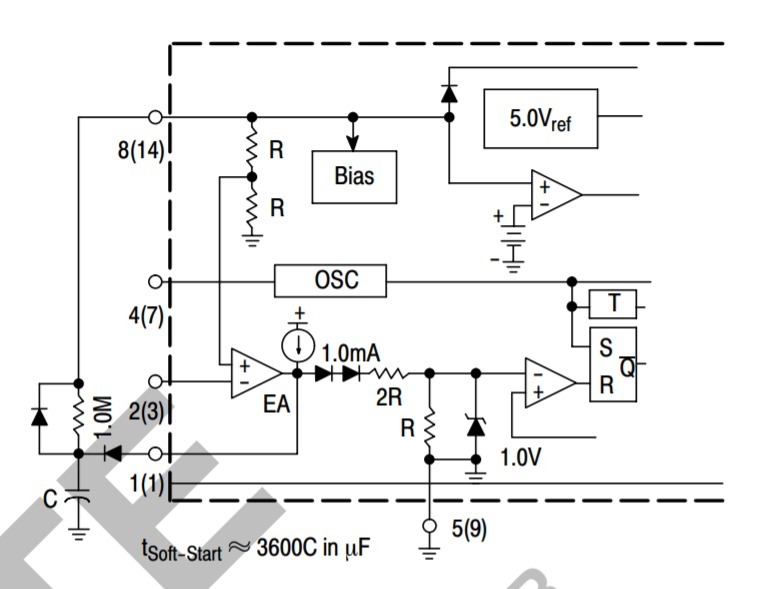
\includegraphics[width=0.5\linewidth]{ic.jpeg}
    \caption {Soft starting circuity of UC3884}
    \label{fig:soft}
\end{figure}
\subsection{Isolation}
Since we will implement isolated DC-DC converters, breaking that isolation brings negative points. However, we should use feedback from output to input in order to obtain voltage control feedback. For that reason, we are planning to use TLP250 optocoupler between output feedback and UC3844.
\section{Cost Analysis}
\begin{table}[H]
    \centering
    \begin{tabular}{|c|c|c|}
    \hline
    Component                                                        & Quantity & \begin{tabular}[c]{@{}c@{}}Cost\\ Euro\end{tabular} \\ \hline
    DPG10I200PM                                                      & 3        & 3.75                                                \\ \hline
    \begin{tabular}[c]{@{}c@{}}CG3885-ALB\\ Inductor\end{tabular}    & 1        & 5.87                                                \\ \hline
    \begin{tabular}[c]{@{}c@{}}860080675012\\ Capacitor\end{tabular} & 1        & 0.4                                                 \\ \hline
    IRF 740N                                                         & 1        & 1                                                   \\ \hline
    0R45959EC Core                                                   & 1        & 5                                                   \\ \hline
    Wire AWG                                                         & -        & 2                                                   \\ \hline
    UC 3844                                                          & 1        & 1     \\ \hline
    ATS-PCB1020                                                      & 1        & 4                                               \\ \hline
    Total Cost                                                       &          & 23                                                  \\ \hline
    \end{tabular}
    \caption{Cost Table}
    \end{table}
\section{References}
\printbibliography
\end{document}
